\chapter{Design}

\section{Overall System Design}

\subsection{Short description of the main parts of the system} 

\begin{itemize}
	\item Assignment Manager
	\begin{itemize}
		\item General User Interface
		\item Display Tasks
		\item Enter new task
		\item Create new 'custom tag'
		\item Complete task
	\end{itemize}
\end{itemize}

\textbf{General User Interface}

The User Interface will display 3 main sections: A Tree View to the left of the central widget, a Table View in the centre, and a section to the right of the screen for a detailed view of particular tasks or processes. There will also be several menus in the menu bar. For example, there will be one called 'File' which will contain all the functions such as 'Open' and 'Save'.

The Tree View will be of a similar design to that of the Tree View in Windows Explorer, the program for Windows 7 that allows you to view your files. It will display all the opened Projects, and those Projects will expand to display all of the attributes, or 'tags', of the tasks within those Projects. For example, if a given user has three on going Projects, Project A, Project B and Project C, each with three Tasks, the Tree View will look something like figure \ref{fig:TreeViewExample}.

\begin{figure}[H]
    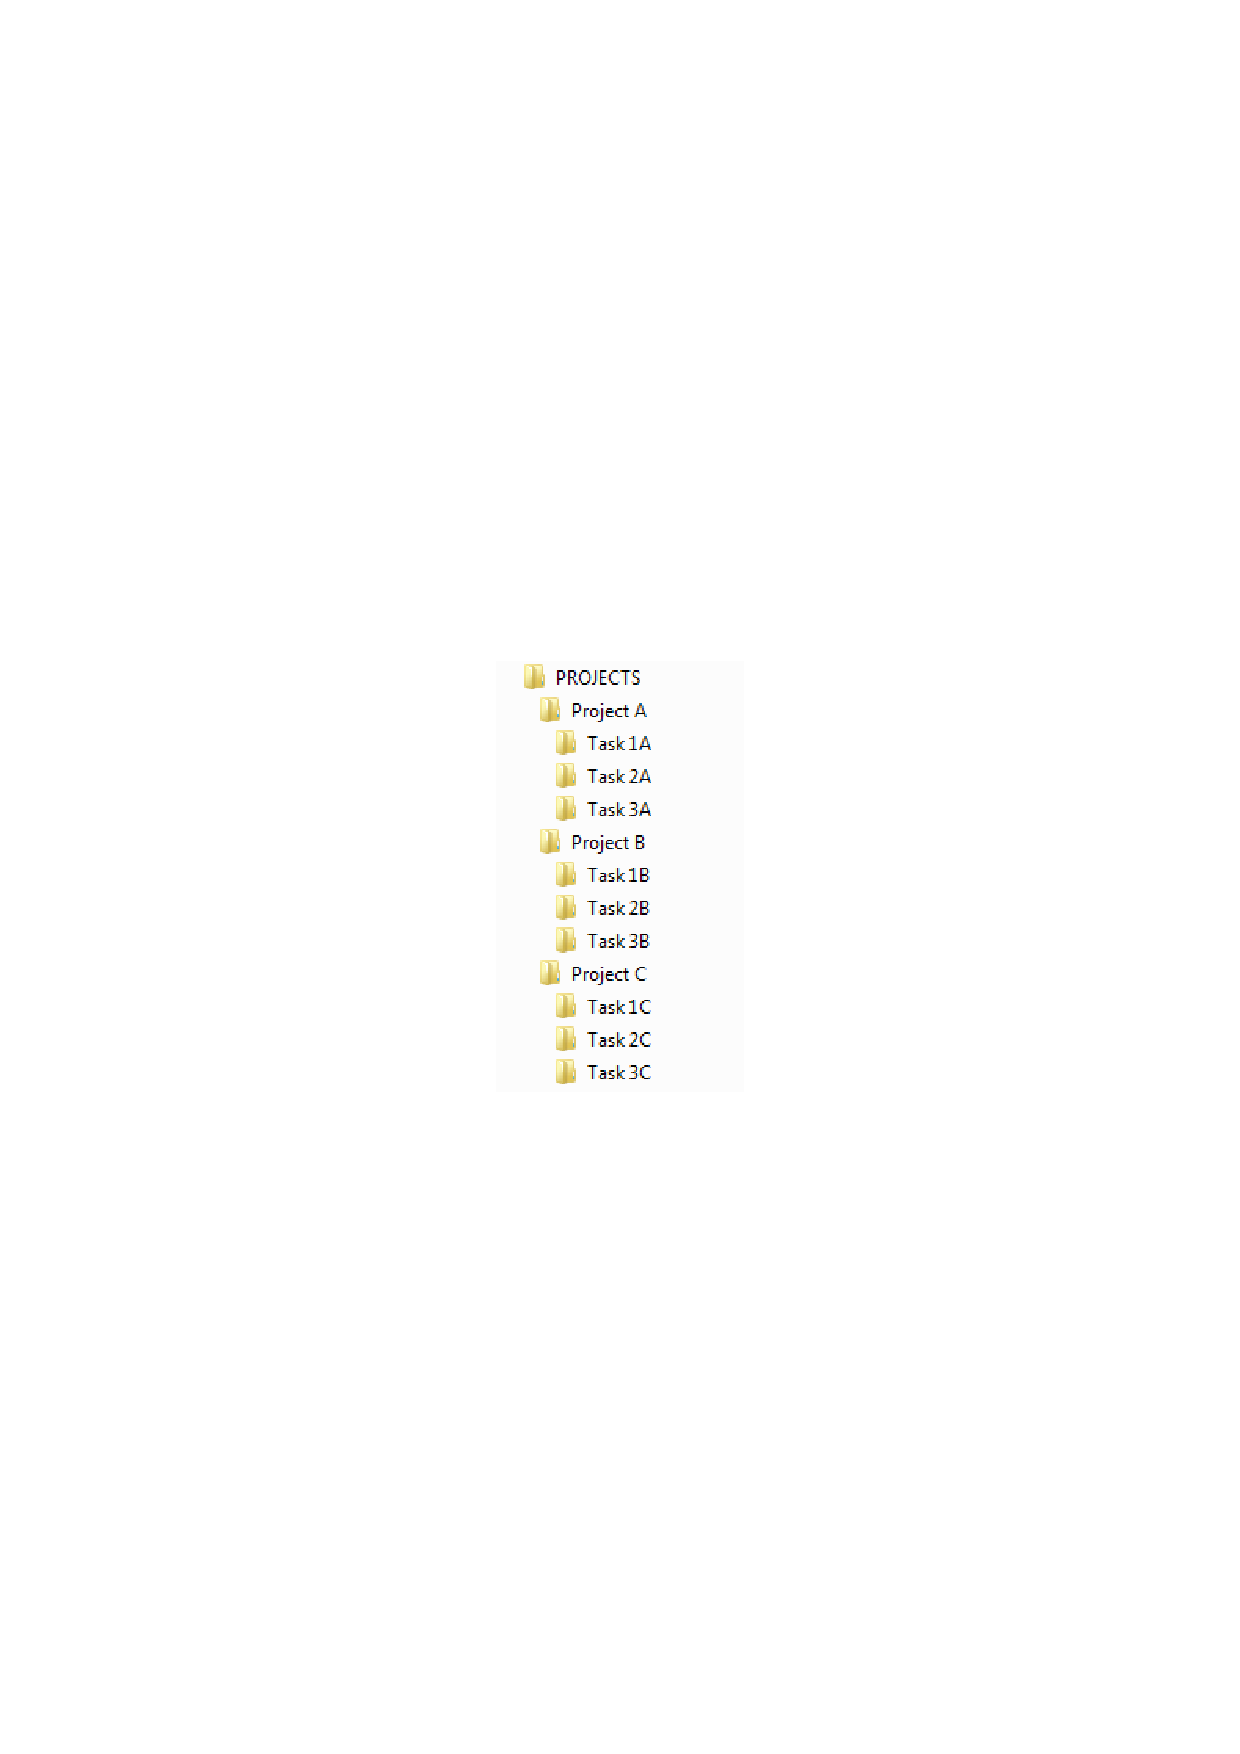
\includegraphics[width=\textwidth]{./Design/Tree_View_Example.pdf}
    \caption{An example Tree View, with three Tasks for each Project. } \label{fig:TreeViewExample}
\end{figure}

The Table View will be where most of the information is displayed on the screen. When loading a Project, by selecting from the Tree View (see figure \ref{fig:TreeViewExample}), All of the Tasks in that Project will be displayed, by default, in order of their unique identifier. Once any given Project is loaded, the default view will be with the attributes (each column will represent an attribute of a given Task) in a logical order from right to left, with the unique identifier being the leftmost column. This is important, as the leftmost column is the column that all the displayed Tasks will be ordered by. When a column heading is clicked and dragged across until it is the leftmost column, the Tasks will be rearranged in order of the new leftmost column. All 'custom' attributes/tags will be displayed last, and in alphabetical order of each other. 

Another way in which the central Table View can be changed is by applying 'filters'. For example, if a Project has 20 Tasks, each with a unique identifier, a due date, a client and a priority, you will be able to apply a filter which gets rid of any Tasks that don't have a particular value for their client. This will enable you to change the Table View to only display tasks set by 'John Smith', for example, or to only display tasks that are due to be completed on a certain day.

\begin{figure}[H]
    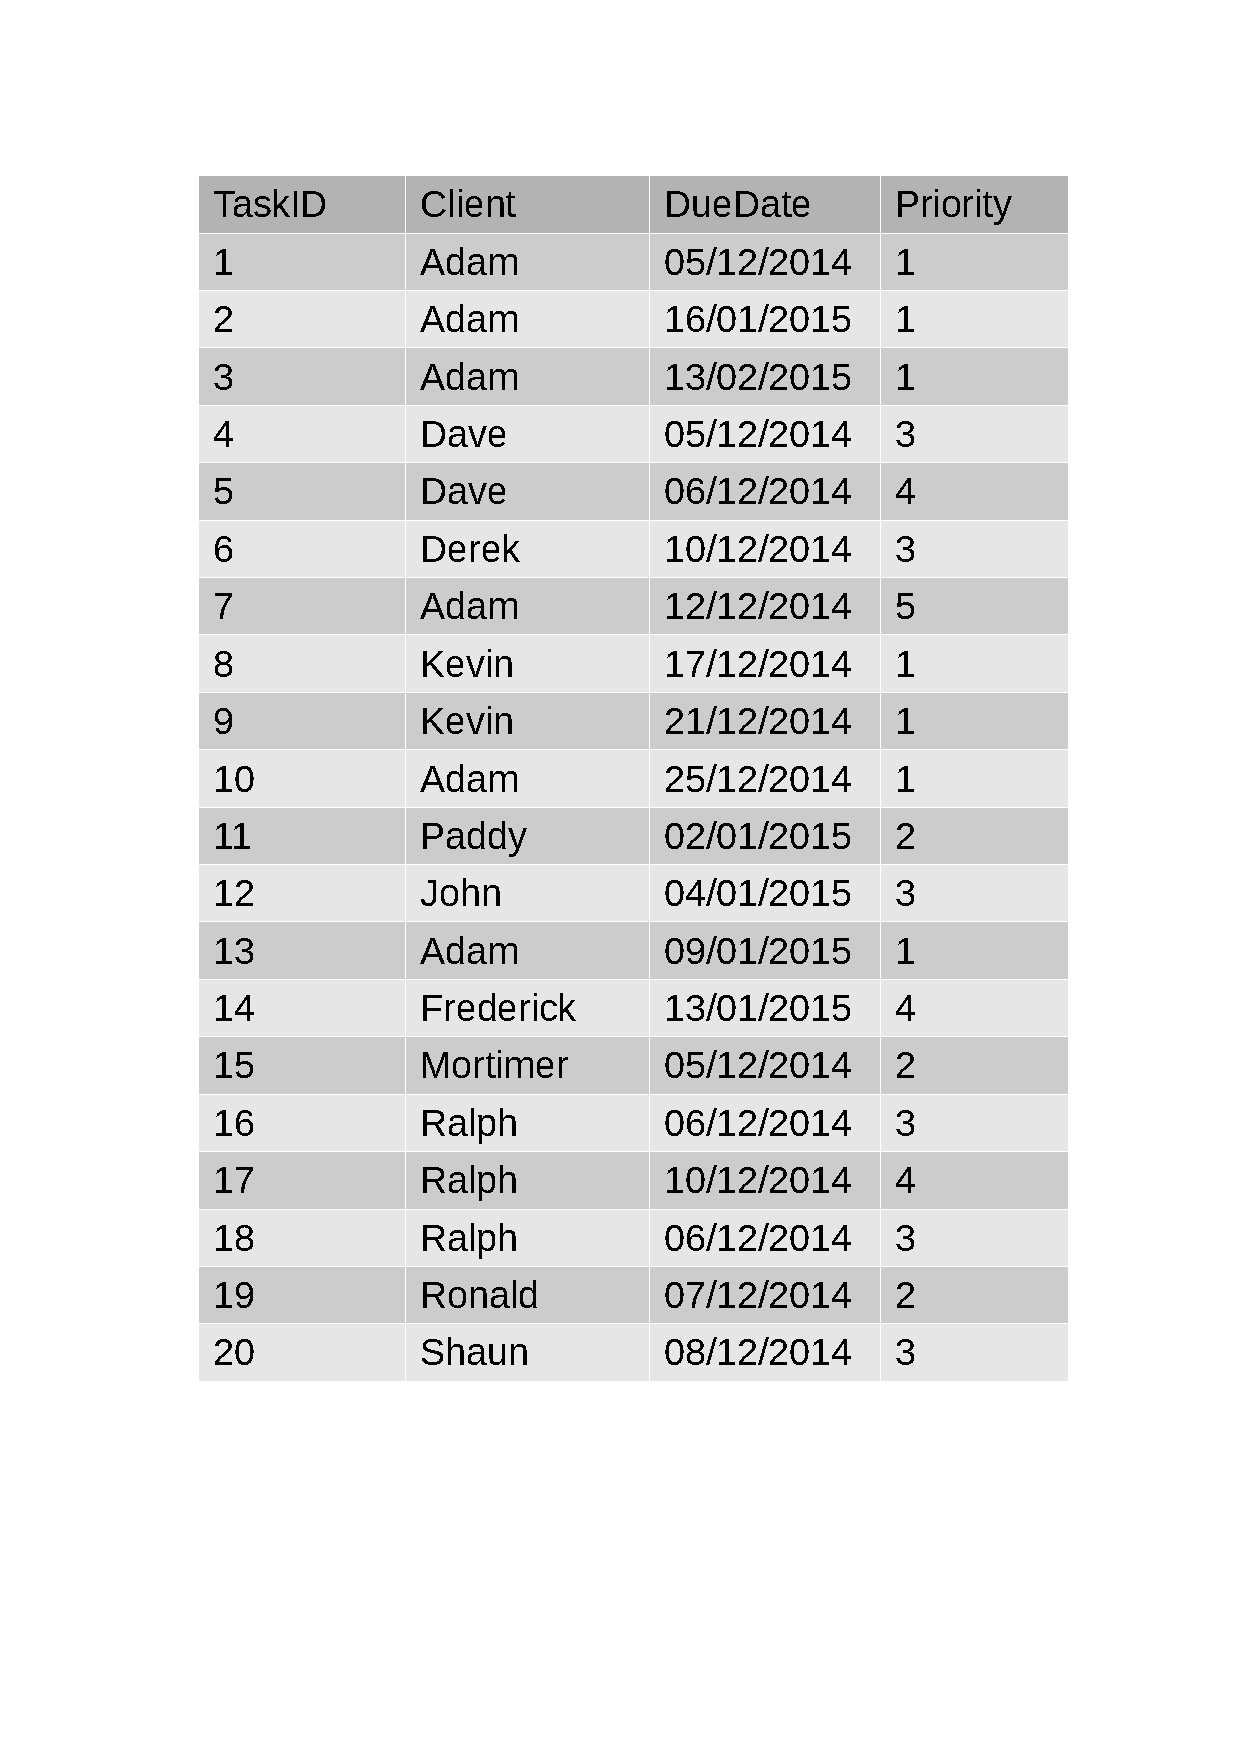
\includegraphics[width=\textwidth]{./Design/Table_View_Example.pdf}
    \caption{An example of a Table View with all Tasks displayed. } \label{fig:TableViewExample}
\end{figure}

\begin{figure}[H]
    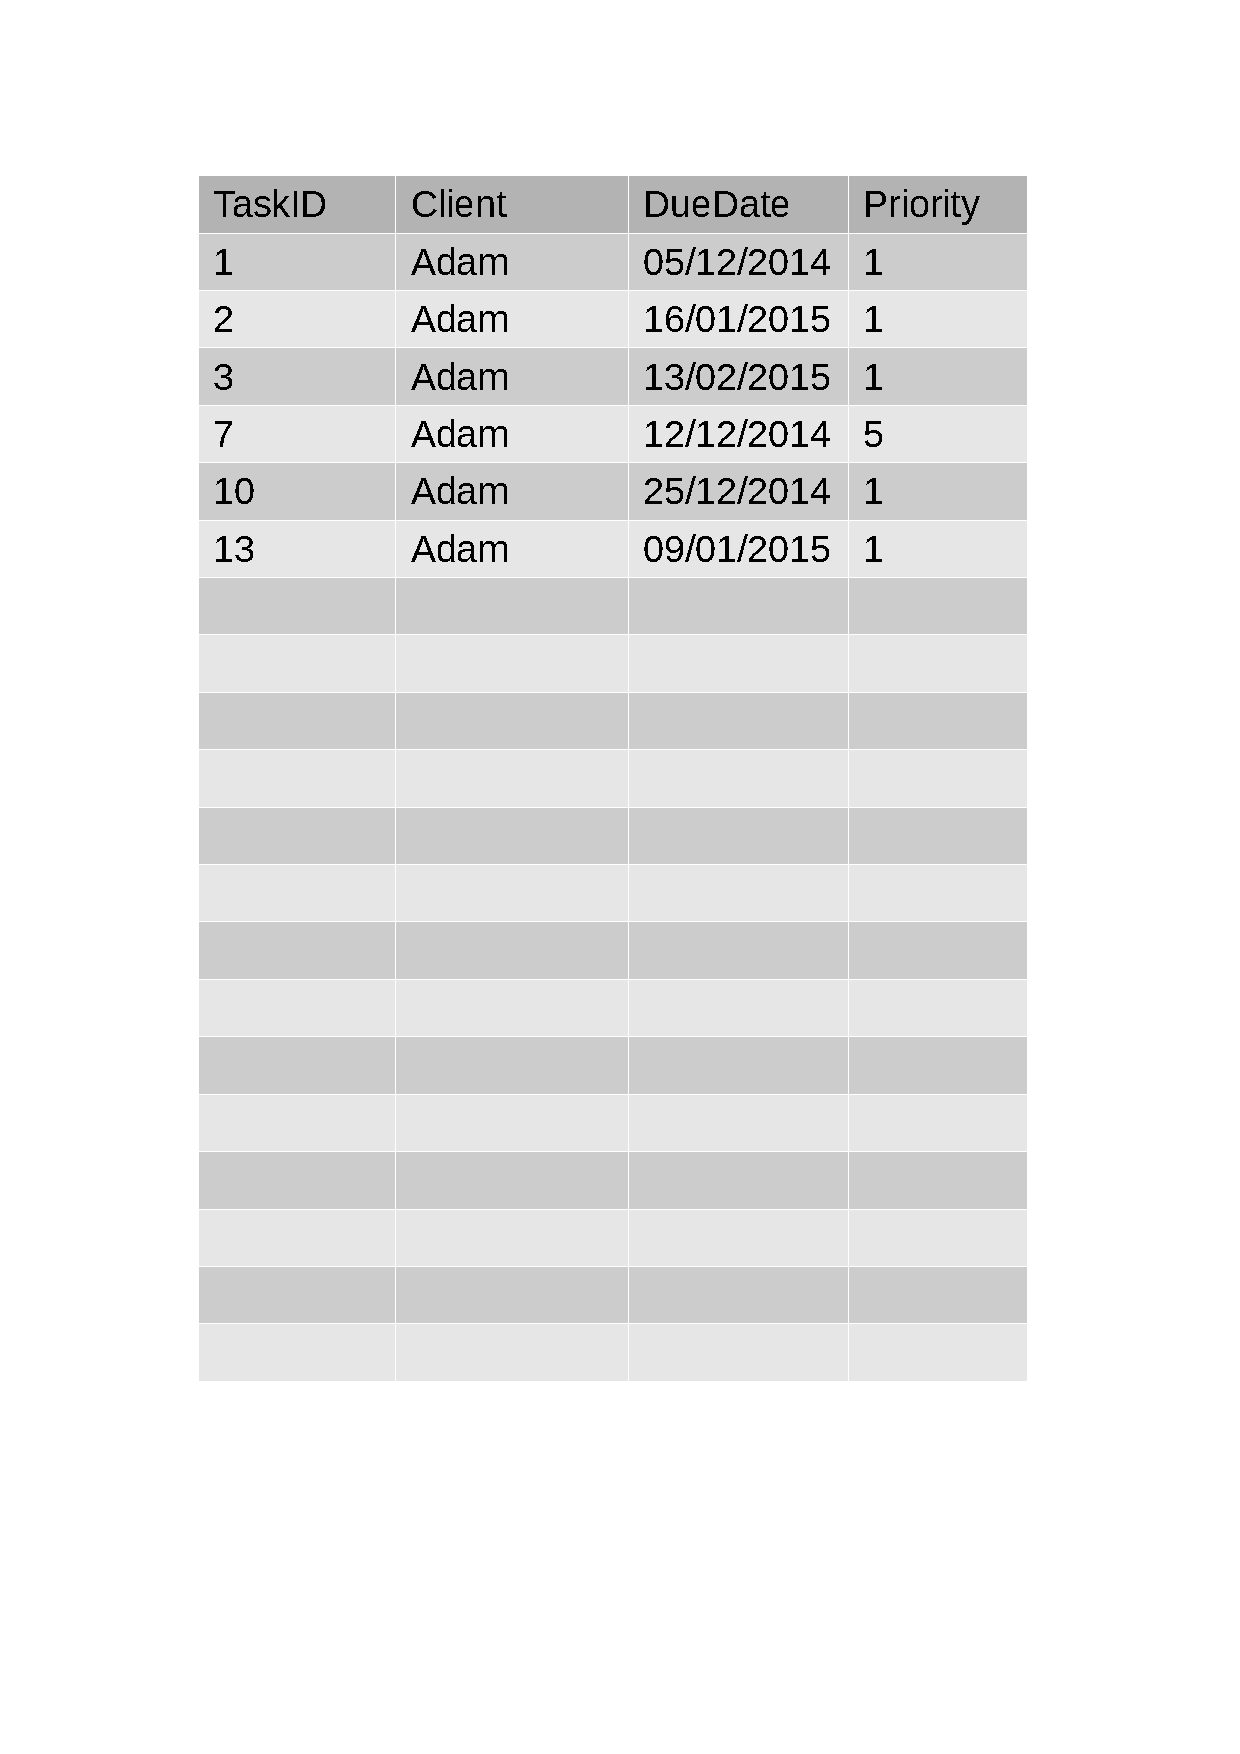
\includegraphics[width=\textwidth]{./Design/Table_View_Example_with_filter.pdf}
    \caption{An example of a Table View with the 'Client: Adam' filter applied. } \label{fig:TableViewExampleWithFilter}
\end{figure}

\textbf{Display Tasks}

When a Project is selected to be loaded, the application will connect with my database, and select all Tasks with that Project attribute. Each Task will then have its attributes added to a list, in order to keep a temporary record of all attributes that need to be displayed. This is necessary because of the possiblity of customisable tags within any given Project. All default attributes will be loaded into the central Table View as column headings from left to right, the leftmost being the unique identifier, and the non-default attributes will be loaded after this, in alphabetical order. The rest of the table will then be poulated with the values of the attributes. All attributes will be displayed, EXECPT for the one that refers to whether a Task is completed or not. Also, if this attribute is read to be True, the Task will be popped from the Table View. 

\textbf{Enter New Task}

Upon selecting the 'add new task to project' function, whether that be from the menu bar or from an icon in the tool bar, a dialogue box will be instatiated, and will prompt the user to enter values for the new Tasks default attributes. The user will then be asked whether they would like to add any custom attributes to the Task, and the user will select from a list of the custom attrbiutes that are already assigned to the Project. After all the required information has been entered by the user, the application will connect with my database, and add the new data to it. This will also require the main Table View to be updated every time a new Task is added to a Project.

\textbf{Create new 'custom tag'}

when the user selects the 'create new custom tag' function, a new column will appear on the Table View, on the right of the table. The heading will be empty, but the user will prompted to enter name for the tag and, optionally, a default value. Once this is done, the application will connect with my database, and update the Project and any Tasks attatched to that Project with the new tag as an attribute, and if necessary, assign that attribute its default value. This will also require the main Table View to be updated every time a new tag is added to a Project.

\textbf{Complete Task}

When a user completes a task, he will be able to select a Task, by clicking the row of that Task, and then select the 'complete Task' function, whether that be from a menu in the menu bar, or an icon in the tool bar. This function will then change the attribute that refers to whether or not the Task is completed, changing it from 'False' to 'True'. this means 

\section{User Interface Designs}

\section{Program Structure}

\subsection{Top-down design structure charts}

\subsection{Algorithms in pseudo-code for each data transformation process}

\subsection{Object Diagrams}

\subsection{Class Definitions}

\section{Prototyping}

\section{Definition of Data Requirements}

\subsection{Identification of all data input items}

\subsection{Identification of all data output items}

\subsection{Explanation of how data output items are generated}

\subsection{Data Dictionary}

\subsection{Identification of appropriate storage media}

\section{Database Design}

\subsection{Normalisation}

\subsubsection{ER Diagrams}

\subsubsection{Entity Descriptions}

\begin{itemize}
	\item Project(\underline{ProjectID}, \emph{CompanyID}, \emph{CustomTagID}, ProjectName)
	\item Task(\underline{TaskID}, \emph{ProjectID}, \emph{ClientID}, DueDate, Priority, TechnicalArea, TaskDescription, TaskDescription, TaskCompleted, \emph{CustomTagID})
	\item Client(\underline{ClientID}, \emph{CompanyID}, ClientFirstName , ClientSecondName, ClientNo)
	\item CustomTag(\underline{CustomTagID}, \emph{TaskID}, TagName, TagValue)
	\item Company(\underline{CompanyID}, CompanyName)
\end{itemize}

\subsubsection{1NF to 3NF}



\section{Security and Integrity of the System and Data}

\subsection{Security and Integrity of Data}

\subsection{System Security}

\section{Validation}

\section{Testing}

\begin{landscape}
\subsection{Outline Plan}

\begin{center}
    \begin{tabular}{|p{2cm}|p{5cm}|p{5cm}|p{4cm}|}
        \hline
        \textbf{Test Series} & \textbf{Purpose of Test Series} & \textbf{Testing Strategy} & \textbf{Strategy Rationale}\\ \hline
        Example & Example & Example & Example \\ \hline
    \end{tabular}
\end{center}

\subsection{Detailed Plan}

\begin{center}
    \begin{longtable}{|p{1.5cm}|p{2.5cm}|p{2.5cm}|p{2cm}|p{2cm}|p{2cm}|p{2cm}|p{2cm}|}
        \hline
        \textbf{Test Series} & \textbf{Purpose of Test} & \textbf{Test Description} & \textbf{Test Data} & \textbf{Test Data Type (Normal/ Erroneous/ Boundary)} & \textbf{Expected Result} & \textbf{Actual Result} & \textbf{Evidence}\\ \hline
        Example & Example & Example & Example & Example & Example & Example & Example \\ \hline
    \end{longtable}
\end{center}
\end{landscape}